\documentclass[12pt]{article}

\usepackage{sbc-template}
\usepackage{graphicx,url}
\usepackage{float}
\usepackage[utf8]{inputenc}
\usepackage[T1]{fontenc}
\usepackage[brazil]{babel}
\sloppy

\title{IoT Distributed: Coleta e Replicação de Leituras em uma Rede de Sensores}

\author{Bruno G. Bitencourt\inst{1}, João M. A. Constâncio\inst{1},
Ramon V. S. Corrêa\inst{1}}

\address{Engenharia de Computação -- PUC Minas\\
Computação Distribuída -- 2026.2\\
Prof. Luigi D. C. Soares}

\begin{document}
\maketitle

\begin{abstract}
This paper describes an IoT project with three processing nodes and independent
PostgreSQL databases. Readings received through MQTT are stored by the node
responsible for each sensor and replicated through gRPC. An HTTP API allows
users to check measurements and identify missing replicas. A .NET simulator
provides readings for the demonstration, while optional ESP32 firmware uses
NTP to synchronize its clock. We describe the architecture, implemented
requirements, and ways to check the data stored in each database.
\end{abstract}

\begin{resumo}
Neste trabalho, desenvolvemos um protótipo IoT com três nós e bancos PostgreSQL
independentes. As leituras chegam por MQTT, são gravadas pelo nó responsável e
enviadas aos demais por gRPC. Uma API HTTP permite consultar os registros e
identificar cópias ausentes. A demonstração usa um simulador .NET; há também
um firmware opcional para ESP32 que sincroniza seu relógio por NTP.
Apresentamos a arquitetura, os recursos implementados e a verificação dos
dados em cada banco.
\end{resumo}

\section{Problema e objetivo}

Quando um sistema recebe dados de vários sensores, é importante conseguir
consultar as leituras armazenadas mesmo após a parada de um processo. A
partir dessa situação, desenvolvemos um protótipo que recebe medições de
temperatura, pressão e nível e as replica entre três nós, cada um com seu
banco de dados. Assim, podemos acompanhar a troca de mensagens e verificar pela
API em quais bancos cada leitura foi gravada. No Docker Compose, os
contêineres são processos separados na mesma máquina.

Usamos \texttt{TEMP-001} (nó 1), \texttt{PRESS-001} (nó 2) e
\texttt{LEVEL-001} (nó 3). No perfil \texttt{demo}, o simulador .NET publica
leituras a cada cinco segundos. Para a demonstração com ESP32 físico, o
firmware gera valores simulados e sincroniza o relógio por NTP. O código está em
\url{https://github.com/brunogbitencourt/IoTDistributed}.

\section{Arquitetura e armazenamento}

O publicador envia ao broker EMQX uma mensagem MQTT em JSON com
\texttt{event\_id} (UUID), \texttt{sensor\_id}, \texttt{value} e
\texttt{collected\_at\_utc}. Cada nó consulta o cadastro de sensores em seu
banco e assina os tópicos MQTT sob sua responsabilidade.

Ao receber a mensagem, o nó valida o identificador, valor, data, sensor e
tópico. Depois grava a leitura em \texttt{sensor\_readings} e envia cópias
por gRPC. Por exemplo, \texttt{TEMP-001} publica em
\texttt{iot/sensors/TEMP-001/readings}: o nó 1 grava em \texttt{db1} e solicita
cópias aos nós 2 e 3, ligados a \texttt{db2} e \texttt{db3}.

O destinatário confere se a origem corresponde ao proprietário do sensor
antes de gravar a cópia. A chave primária \texttt{event\_id} e o comando
\texttt{ON CONFLICT DO NOTHING} evitam duplicatas no mesmo banco; o mesmo
UUID nos três bancos representa as cópias esperadas.

Cada banco PostgreSQL possui a tabela \texttt{sensors}, com o nó proprietário e o
tópico de cada sensor. O serviço \texttt{db-init} executa os scripts SQL que
criam e preenchem as tabelas nos três bancos, mantidos em volumes Docker
separados.

Cada registro de \texttt{sensor\_readings} guarda o UUID, sensor, valor,
horário de coleta e nó de origem. O banco preenche \texttt{created\_at} na
inserção, permitindo distinguir o instante da persistência do horário da
medição.

O Compose inicia os nós após os testes de saúde dos bancos e a conclusão do
\texttt{db-init}. Na pasta \texttt{src/IoTDistributed.Node}, executamos
\texttt{docker compose -{}-profile demo up -d -{}-build}. A API ASP.NET Core
consulta os três PostgreSQL, enquanto o dashboard acessa a API. A
Figura~\ref{fig:arquitetura} resume esse fluxo.

\begin{figure}[!htbp]
\centering
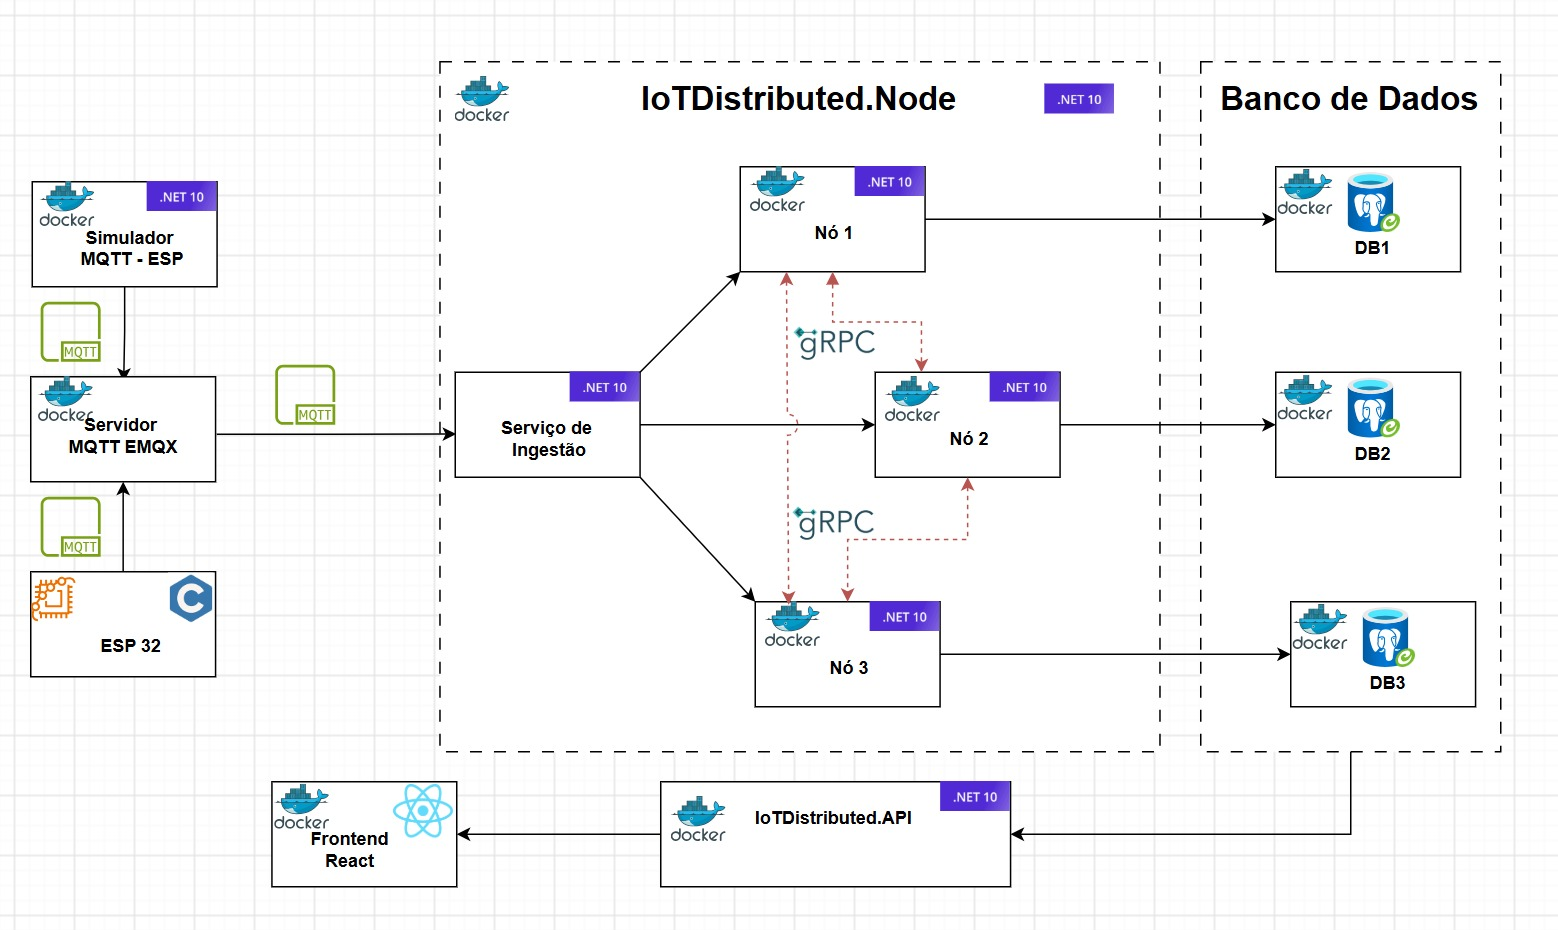
\includegraphics[width=.82\textwidth]{images/diagrama-projeto.jpeg}
\caption{Visão conceitual do sistema: a ingestão ocorre nos nós; o simulador
.NET e o ESP32 são alternativas para publicar medições.}
\label{fig:arquitetura}
\end{figure}

\section{Requisitos de computação distribuída}

\subsection{RPC com gRPC}

A comunicação entre os nós usa gRPC sobre HTTP/2. Cada um oferece
\texttt{SubmitReading}, que recebe uma medição no nó responsável;
\texttt{ReplicateReading}, que recebe a cópia e verifica a origem; e
\texttt{Ping}, para chamadas pontuais de comunicação.

Depois de salvar uma leitura nova, o nó chama os dois pares em paralelo,
com prazo de três segundos por chamada. O serviço registra as confirmações
e eventuais erros nos logs, preservando a leitura gravada localmente.

\subsection{Web services HTTP}

Para consultar o sistema, desenvolvemos uma API REST com as rotas
\texttt{GET /api/sensors}, \texttt{GET /api/readings},
\texttt{GET /api/readings/\{eventId\}/replicas},
\texttt{GET /api/cluster/databases}, \texttt{GET /api/cluster/health} e
\texttt{GET /api/replication/divergences}. Na consulta de leituras, usamos
os filtros \texttt{node}, \texttt{limit} e \texttt{sensorId}.

Ao consultar um \texttt{eventId}, a API verifica os três bancos e retorna
\texttt{present} para uma cópia encontrada, \texttt{missing} para uma cópia
ausente em banco acessível e \texttt{unavailable} para um banco indisponível.
Assim, distinguimos falta de registro de falha de acesso.

A rota \texttt{GET /api/replication/divergences} considera, por padrão,
leituras dos últimos 15 minutos e aceita janelas UTC de até uma hora.
A API reúne os UUIDs dos bancos acessíveis em um conjunto e compara esse
resultado com os registros de cada banco para identificar os ausentes.

Um evento presente em \texttt{db1} e \texttt{db2}, mas ausente em
\texttt{db3}, será apontado como divergente. Se \texttt{db3} estiver
indisponível, a comparação será marcada como parcial. As rotas de saúde
da API e de disponibilidade dos bancos verificam estados diferentes.

\subsection{Relógio físico no firmware opcional}

No firmware do ESP32, o dispositivo consulta um servidor NTP após conectar
ao Wi-Fi e usa o horário UTC em \texttt{collected\_at\_utc}. Esse fluxo
pode ser demonstrado com o dispositivo físico.

No Docker, o simulador .NET usa \texttt{DateTimeOffset.UtcNow} para publicar
medições. Com esse ambiente, apresentamos o funcionamento do gRPC e dos web
services HTTP; a demonstração NTP utiliza o ESP32.

\section{Interface web de monitoramento}

Desenvolvemos um frontend em React para acompanhar os dados retornados pela
API. Na tela \emph{Visão geral} (Figura~\ref{fig:frontend}), vemos o número de sensores cadastrados, a
disponibilidade dos três bancos e as leituras mais recentes de temperatura,
pressão e nível. Também podemos selecionar um sensor para consultar seu
histórico e acompanhar as últimas medições. O painel atualiza as informações
periodicamente, facilitando a observação dos dados publicados pelo simulador.

O menu lateral organiza as telas de \emph{Medições}, \emph{Infraestrutura} e
\emph{Replicação}. Com elas, podemos inspecionar os registros, verificar o
estado dos bancos e observar as divergências identificadas pela API. O
frontend consulta a API HTTP; a gravação e a replicação das leituras ficam a
cargo dos nós.

\begin{figure}[H]
\centering
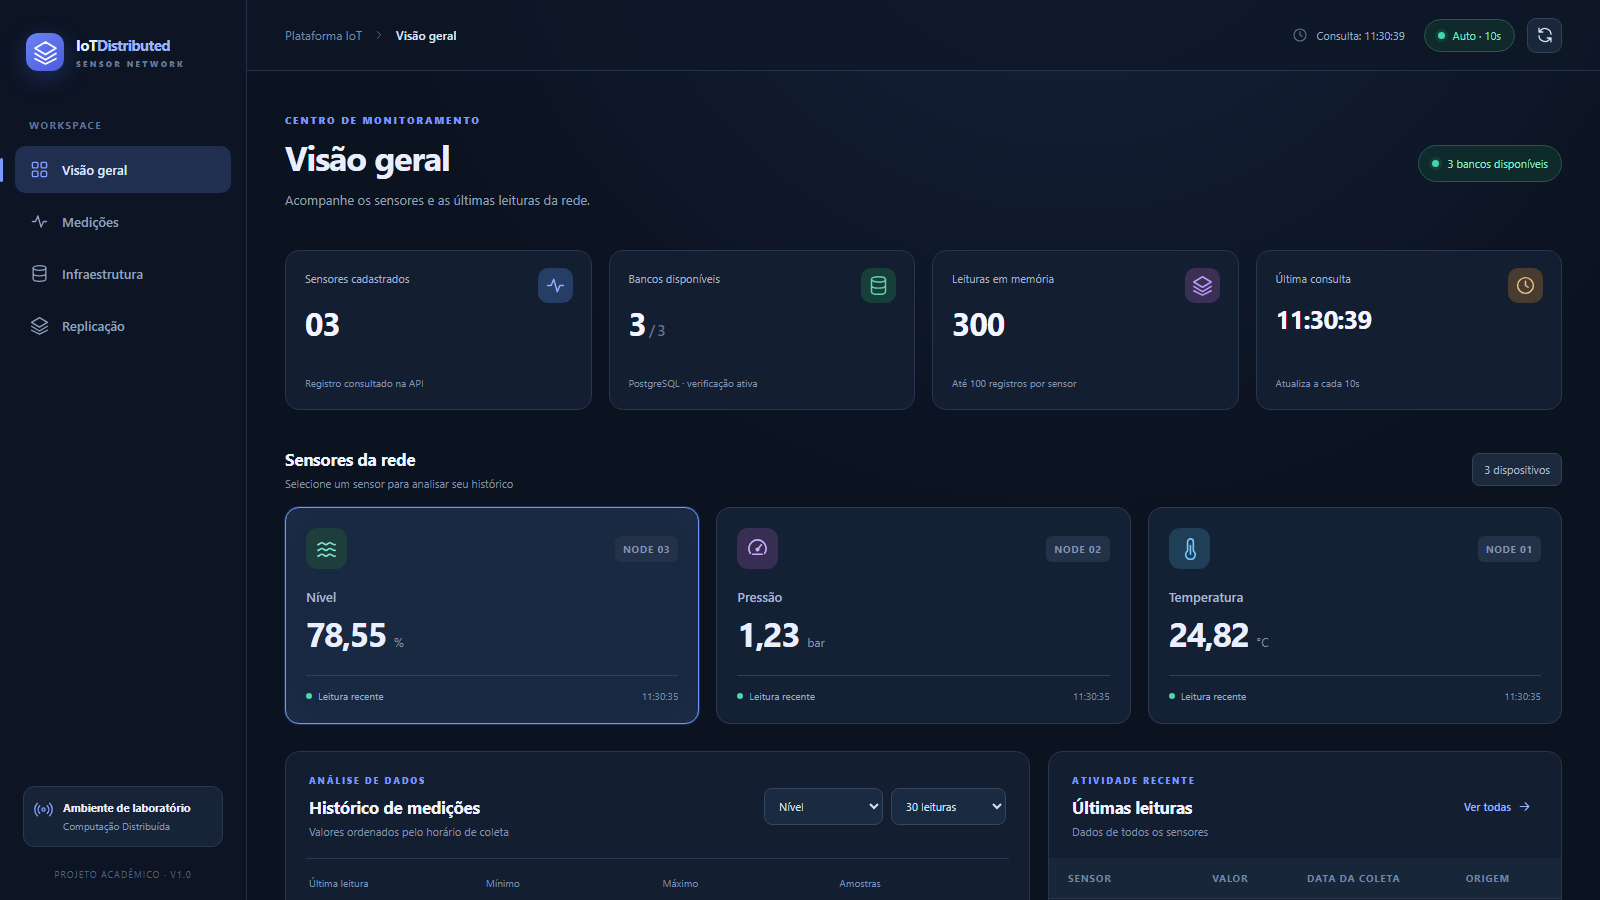
\includegraphics[width=.56\textwidth]{images/frontend-visao-geral.png}
\caption{Tela Visão geral do frontend, com estado dos bancos e leituras dos sensores.}
\label{fig:frontend}
\end{figure}

\section{Desafios e verificação da primeira entrega}

Durante o desenvolvimento, cuidamos da ordem de inicialização dos bancos,
scripts e nós por meio das dependências e verificações de saúde do Compose.
Também tratamos mensagens repetidas do MQTT com QoS 1: o UUID e
\texttt{ON CONFLICT DO NOTHING} evitam duplicatas em cada banco.

Outro cuidado foi tornar visível a replicação: os logs mostram envios e
erros de comunicação, enquanto a API permite conferir as cópias encontradas
em cada banco.

Para observar falhas, podemos parar \texttt{node-3} mantendo \texttt{db3}
ativo: a API ainda consulta esse banco. Ao parar \texttt{db3}, a comparação
é parcial. Após reiniciar os serviços, consultamos novamente as cópias.

Para conferir os dados, iniciamos o perfil \texttt{demo}, consultamos
\texttt{GET /api/readings?node=1\&limit=20} e usamos um \texttt{eventId}
na rota de réplicas. A consulta de divergências mostra diferenças por período;
republicar o mesmo UUID permite verificar a prevenção de duplicatas.

Na apresentação, os logs mostram as publicações, a gravação e as respostas
gRPC. O dashboard reúne as leituras, o estado dos bancos e as divergências.

\section{Participação dos integrantes}

\begin{itemize}
\item \textbf{Bruno Guimarães Bitencourt}: configuração da infraestrutura
Docker/Compose, dos bancos PostgreSQL e dos scripts usados para criar as
tabelas e cadastrar os sensores.
\item \textbf{João Miguel de Abreu Constâncio}: implementação da recepção de
mensagens MQTT, das validações e da replicação por gRPC, além da colaboração
na redação das partes de arquitetura e requisitos.
\item \textbf{Ramon Vinícius Silva Corrêa}: desenvolvimento da API de
consulta, integração com o simulador ESP32 e organização e revisão do
relatório.
\end{itemize}

\section{Considerações finais}

Nesta primeira entrega, reunimos MQTT para receber medições, gRPC para
compartilhá-las entre os nós e uma API HTTP para consultar os bancos. Com
isso, demonstramos os requisitos de RPC e web services no ambiente Docker.
A sincronização NTP está presente no firmware opcional para ESP32 físico.

\end{document}
